
\documentclass[11pt,a4paper]{article}
\usepackage[margin=0.82in]{geometry}
\usepackage{amsmath,amsfonts,amssymb,bm}
\usepackage{graphicx}
\usepackage{booktabs}
\usepackage{tabularx}
\usepackage{array}
\usepackage{longtable}
\usepackage{multirow}
\usepackage{hyperref}
\usepackage{xcolor}
\usepackage{enumitem}
\usepackage{caption}
\usepackage{subcaption}
\usepackage{float}
\usepackage{microtype}
\usepackage[T1]{fontenc}
\usepackage[utf8]{inputenc}

\definecolor{mmalsblue}{HTML}{1F4E79}
\definecolor{mmalsteal}{HTML}{0F766E}
\definecolor{mmalsgray}{HTML}{374151}
\hypersetup{colorlinks=true, linkcolor=mmalsblue, citecolor=mmalsteal, urlcolor=mmalsblue}

\title{\textbf{Goal-Adaptive MMALS: A Geometry/RL/Forward-Backward Extension of RC2O for Objective-Conditioned Routing}\\
\large Synthetic Smoke Evidence and Reproducibility Package}
\author{Anonymous for review\\\small MMALS experimental research note}
\date{June 2026}

\begin{document}
\maketitle

\begin{abstract}
Multi-host continual learning systems require more than final accuracy: they must retain past functions, route inputs through specialized hosts, remain stable under drift, and expose auditable trade-offs between performance and cost. This article presents a goal-adaptive extension of the MMALS RC2O selector. The validated core is treated as a continual-learning routing scaffold, while three additional layers are instrumented: an audit geometry over context-route-host-memory features, a reinforcement-learning meta-router over routing actions, and an Ollivier-style forward-backward view in which each route is scored by the future functional state it makes reachable. We evaluate the extension on controlled synthetic traces over an 8-dataset RC2O-style scaffold. The experiment tests five explicit objectives: accuracy, retention, cost, drift stability, and host specialization. The main result is not a claim of real 8-dataset superiority. Rather, the smoke run demonstrates that, under identical audit states, different objective vectors induce different routing policies: accuracy goals select accuracy specialists, retention goals remain close to conservative RC2O routing, cost goals select cheaper routes, drift goals select stabilizing routes, and specialization goals select host-specializing routes. The package includes the Colab notebook, all generated CSV files, all figures, and this compiled article.
\end{abstract}

\noindent\textbf{Reviewer caveat.} This is a smoke/synthetic trace report. It validates the experimental instrumentation and the goal-conditioned route-differentiation mechanism. It does not replace real RC2O-8D training/evaluation evidence, and it does not claim that MMALS is already a proven universal controller.

\section{Motivation}
Continual learning (CL) asks whether a model can learn a sequence of tasks without catastrophic forgetting. In the MMALS setting, the problem is richer: multiple hosts or heads can carry partially specialized functions, and a selector must route each state toward a suitable candidate. The existing RC2O selector is therefore best interpreted as a transparent continual-learning selector over candidate traces.

However, once routing is available, a second question appears. The system may not always want the same route. In one situation, it may prioritize immediate accuracy; in another, it may prioritize retention of previous tasks, stability under drift, low cost, or explicit host specialization. This suggests a control problem over routing decisions.

The goal of this work is to make that control problem testable. We keep the RC2O backbone as the validated continual-learning core, and add a read-only, post-hoc controller that chooses among candidate routes according to a current objective. The central hypothesis is:

\begin{quote}
\emph{If MMALS routing can be lifted from static selection to goal-conditioned control, then identical states should induce different route distributions under different objective vectors.}
\end{quote}

This is the claim evaluated in the smoke run.

\section{Positioning}
\subsection{Continual learning core}
CL studies adaptation under sequential tasks and the prevention of forgetting. Representative approaches include regularization-based methods such as Elastic Weight Consolidation \cite{kirkpatrick2017ewc}, distillation approaches such as Learning without Forgetting \cite{li2016lwf}, gradient and episodic-memory approaches \cite{lopezpaz2017gem}, replay-based methods, and architecture expansion methods such as Progressive Neural Networks \cite{rusu2016pnn}. In the MMALS roadmap, RC2O is positioned as a selector over candidate traces rather than as an end-to-end raw-pixel continual learner.

\subsection{Geometry-aware interpretation}
The geometry layer is motivated by the observation that many learning and filtering problems are not naturally Euclidean. Riemannian and Lie-group-aware filtering and learning methods preserve constraints when states, observations, or parameters live on structured spaces \cite{labsir2026filtering}. The present work does not claim that the audit space is already a formal Riemannian manifold. Instead, it introduces an \emph{audit geometry}: a structured vector space where route, host, memory, stability, cost, and specialization can be compared and visualized.

\subsection{Control and forward-backward representations}
Reinforcement learning formalizes sequential decision-making through states, actions, rewards, and long-term utility \cite{sutton2018rl}. Universal control and successor-feature methods ask whether one can learn reusable representations of dynamics that support fast adaptation to new rewards \cite{barreto2017successor}. Touati and Ollivier introduce forward-backward representations that aim to learn one representation of reward-free dynamics and then obtain policies for rewards specified a posteriori \cite{touati2021fb}. Related zero-shot RL work clarifies the goal of solving new tasks after reward-free learning \cite{touati2022zeroshot}. We use this idea as a conceptual and experimental layer: each MMALS route is scored by its predicted future vector, and a goal vector selects the route whose reachable future best aligns with the current objective.

\section{Four-layer MMALS extension}
Figure~\ref{fig:conceptual} summarizes the conceptual hierarchy. The extension has four layers.

\begin{figure}[H]
\centering
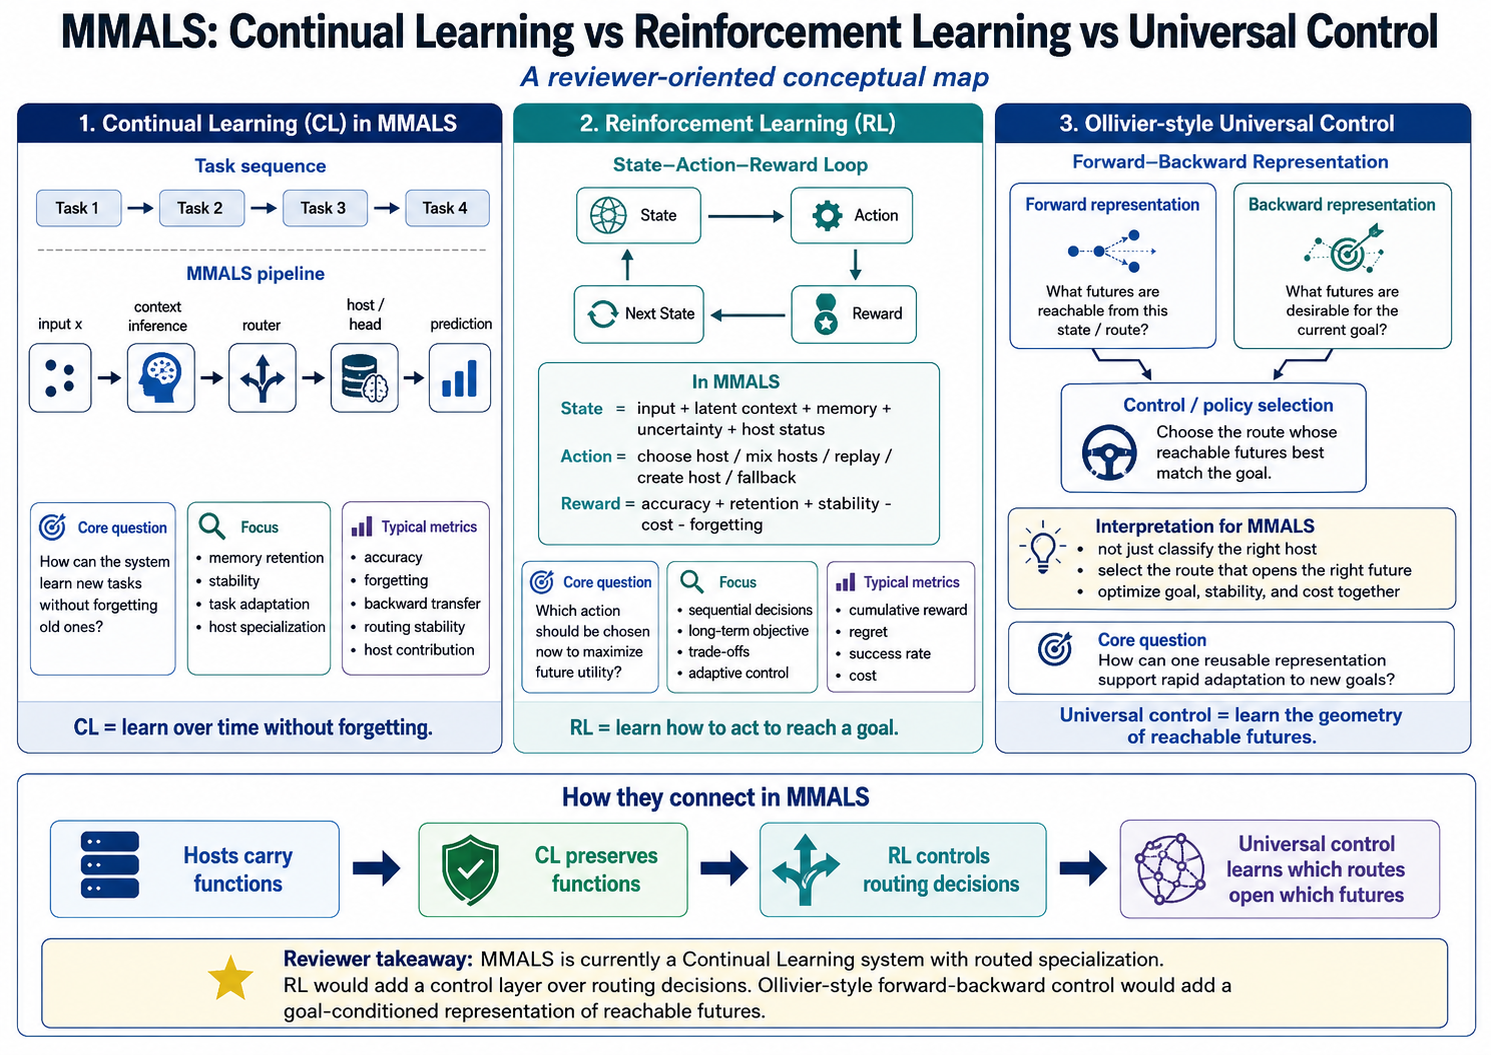
\includegraphics[width=0.95\linewidth]{figures/mmals_cl_rl_fb_conceptual_map.png}
\caption{Conceptual map: CL preserves functions, RL controls routing decisions, and forward-backward control learns which routes open which futures.}
\label{fig:conceptual}
\end{figure}

\subsection{Layer 1: RC2O continual-learning selector}
The RC2O layer selects among candidate traces using auditable metrics. Let $T_1,\ldots,T_K$ be a sequence of tasks or regimes. A candidate $a$ at state $s$ is evaluated through metrics such as accuracy, retention, stability, route entropy, cost, and specialization. A minimal CL objective is:
\begin{equation}
\max_{a} \; \mathrm{Acc}(a) - \lambda_F \mathrm{Forget}(a),
\end{equation}
with post-hoc audit metrics such as final average accuracy, average forgetting, and route stability.

\subsection{Layer 2: MMALS audit geometry}
For each state-action pair, the notebook constructs an audit vector:
\begin{equation}
\phi(s,a) = [\mathrm{accuracy},\mathrm{retention},\mathrm{stability},\mathrm{cost\_good},\mathrm{specialization},\ldots].
\end{equation}
This vector is not treated as a proof of manifold structure. It is a practical coordinate system that allows candidate routes to be compared, visualized, and later replaced by manifold-aware filtering or optimization.

\subsection{Layer 3: RL meta-router}
Routing can be written as a sequential decision problem:
\begin{equation}
S_t = (z_t,m_t,h_t,e_t,d_t), \qquad A_t \in \mathcal{A},
\end{equation}
where $z_t$ is a latent context, $m_t$ a memory state, $h_t$ host status, $e_t$ uncertainty or route entropy, and $d_t$ drift. Actions include using RC2O, using an accuracy specialist, choosing a cost saver, selecting a drift stabilizer, promoting specialization, replaying memory, or triggering a fallback. A generic reward is:
\begin{equation}
R_t = w_A A_t + w_R Ret_t + w_S Stab_t - w_C Cost_t + w_H Spec_t - P_t,
\end{equation}
where $P_t$ collects constraint penalties such as retention violation or instability.

\subsection{Layer 4: Forward-backward universal-control view}
The forward-backward layer uses a simplified alignment score:
\begin{equation}
F(s,a) = [A(s,a), Ret(s,a), Stab(s,a), CostGood(s,a), Spec(s,a)],
\end{equation}
\begin{equation}
B(g) = \text{goal vector for objective }g,
\end{equation}
\begin{equation}
 a^*(s,g) = \arg\max_{a\in\mathcal{A}} \langle F(s,a), B(g) \rangle - \Omega(s,a,g).
 \label{eq:fbscore}
\end{equation}
Here $F(s,a)$ approximates the future made reachable by a route, $B(g)$ encodes the desired future, and $\Omega$ penalizes violations of future-retention, cost, or stability constraints.

\section{Experimental design}
\subsection{Purpose of the smoke run}
The purpose is to test the instrumentation, not to replace real RC2O-8D evidence. The synthetic traces are designed to induce conflicts between objectives. This is required because a goal-adaptive controller can only be evaluated if different goals produce different optimal policies.

\subsection{Objectives}
The five goals are:
\begin{enumerate}[label=\textbf{Goal \Alph*:},leftmargin=*]
    \item maximize accuracy;
    \item maximize retention;
    \item minimize cost;
    \item maximize stability under drift;
    \item maximize host specialization.
\end{enumerate}

Each goal corresponds to a different vector $B(g)$ in Eq.~\ref{eq:fbscore}. The experiment asks whether:
\begin{equation}
 g_i \neq g_j \quad \Rightarrow \quad \pi(\cdot|g_i) \neq \pi(\cdot|g_j),
\end{equation}
where $\pi$ is the induced route-selection distribution.

\subsection{Compared selectors}
The adaptive controller is compared to fixed RC2O under each goal. This produces two quantities: adaptive utility and the utility obtained by replaying the RC2O route under the same goal scoring function.

\section{Results}
\subsection{Goal-conditioned utilities}
Table~\ref{tab:summary} shows the global summary. The adaptive controller improves goal-specific utility over fixed RC2O for all five objectives in the synthetic trace run. The largest improvements occur for cost and host specialization, which are objectives that fixed RC2O was not designed to optimize directly.

\begin{table}[H]
\centering
\scriptsize
\caption{Goal-adaptive smoke summary. Values are synthetic trace results. The key column is the route-change rate versus fixed RC2O, which shows whether the controller changes policy under different goals.}
\label{tab:summary}
\resizebox{\textwidth}{!}{%
\begin{tabular}{llrrrrrrrrr}
\toprule
Goal & Dominant action & Adaptive U & RC2O U & $\Delta$ & Change & Acc. & Ret. & Stab. & Cost & Spec. \\
\midrule
Goal\_A\_accuracy & accuracy\_specialist & 1.632 & 1.607 & 0.026 & 88.1\% & 0.938 & 0.920 & 0.855 & 0.651 & 0.572 \\
Goal\_B\_retention & RC2O\_static & 2.029 & 2.026 & 0.004 & 43.1\% & 0.854 & 0.999 & 0.972 & 0.618 & 0.601 \\
Goal\_C\_cost & cost\_saver & 1.878 & 1.717 & 0.160 & 100.0\% & 0.770 & 0.926 & 0.818 & 0.354 & 0.515 \\
Goal\_D\_stability\_drift & drift\_stabilizer & 2.346 & 2.274 & 0.072 & 87.5\% & 0.823 & 0.999 & 0.999 & 0.638 & 0.577 \\
Goal\_E\_specialization & specialization\_promoter & 1.984 & 1.748 & 0.236 & 100.0\% & 0.855 & 0.955 & 0.886 & 0.653 & 0.808 \\
\bottomrule
\end{tabular}}
\end{table}

\subsection{Route distributions by goal}
Figure~\ref{fig:routes} shows that the controller does not simply reproduce RC2O. Accuracy selects the accuracy specialist, retention remains partly conservative, cost selects the cost saver, drift stability selects the drift stabilizer, and specialization selects the specialization promoter.

\begin{figure}[H]
\centering
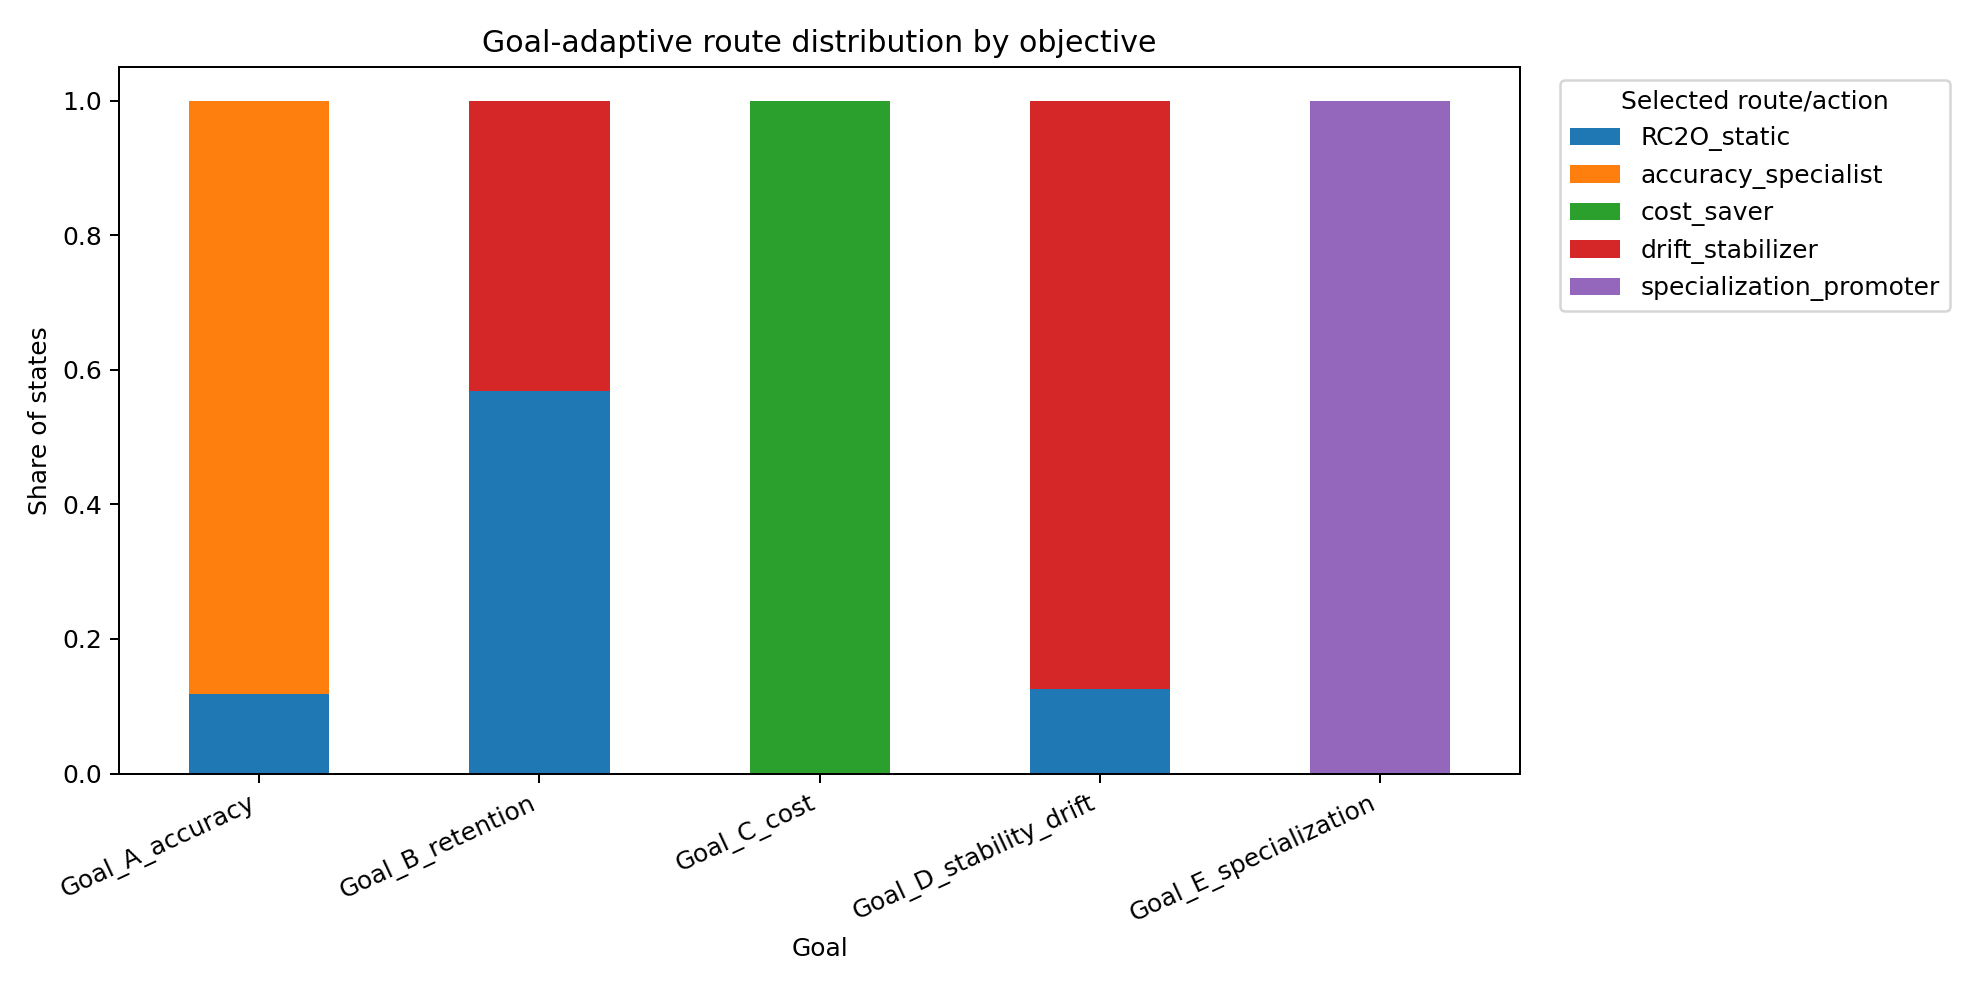
\includegraphics[width=0.95\linewidth]{figures/route_distribution_by_goal.png}
\caption{Route distribution by goal. The dominant route changes with the objective, which is the central smoke evidence for goal-conditioned routing.}
\label{fig:routes}
\end{figure}

\subsection{Utility comparison}
Figure~\ref{fig:utility} compares adaptive goal-conditioned utility against fixed RC2O utility under the same goals. The result supports a modest claim: the controller is able to optimize the scoring function it is given in the controlled synthetic traces.

\begin{figure}[H]
\centering
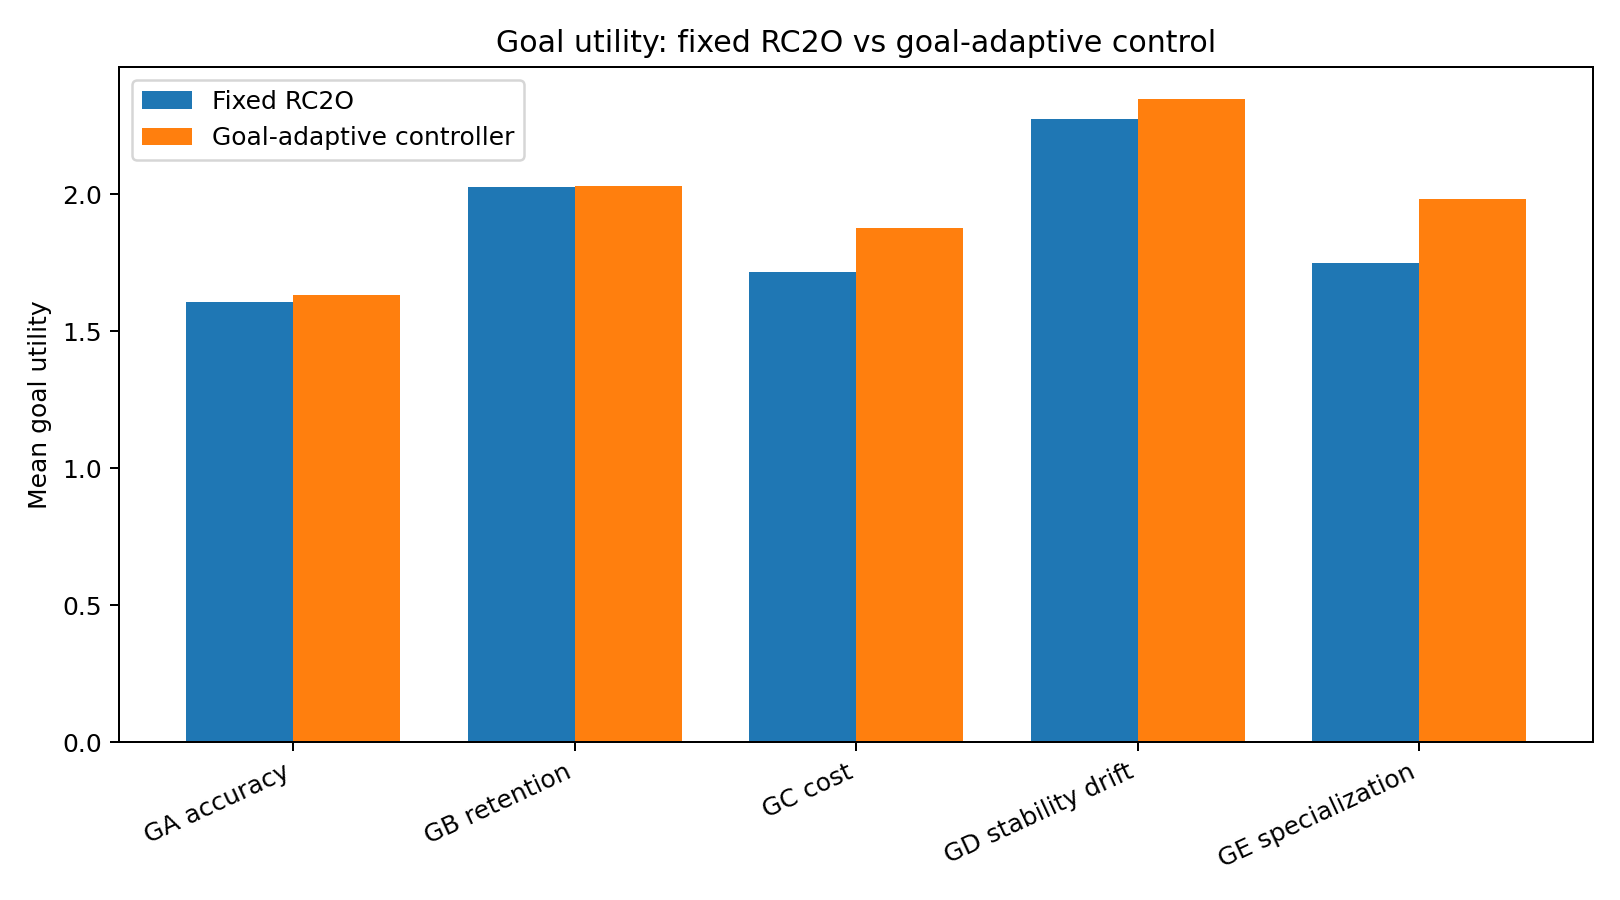
\includegraphics[width=0.85\linewidth]{figures/utility_comparison_by_goal.png}
\caption{Adaptive utility vs fixed RC2O utility under each objective. These are smoke results, not final empirical evidence.}
\label{fig:utility}
\end{figure}

\subsection{Pairwise goal differentiation}
The pairwise route-change heatmap in Figure~\ref{fig:heatmap} is the strongest reviewer-facing result. Several goal pairs induce 100\% route change, including accuracy vs cost, accuracy vs specialization, cost vs drift stability, and drift stability vs specialization. Retention and drift stability overlap partially, which is expected because both favor conservative and stable policies.

\begin{figure}[H]
\centering
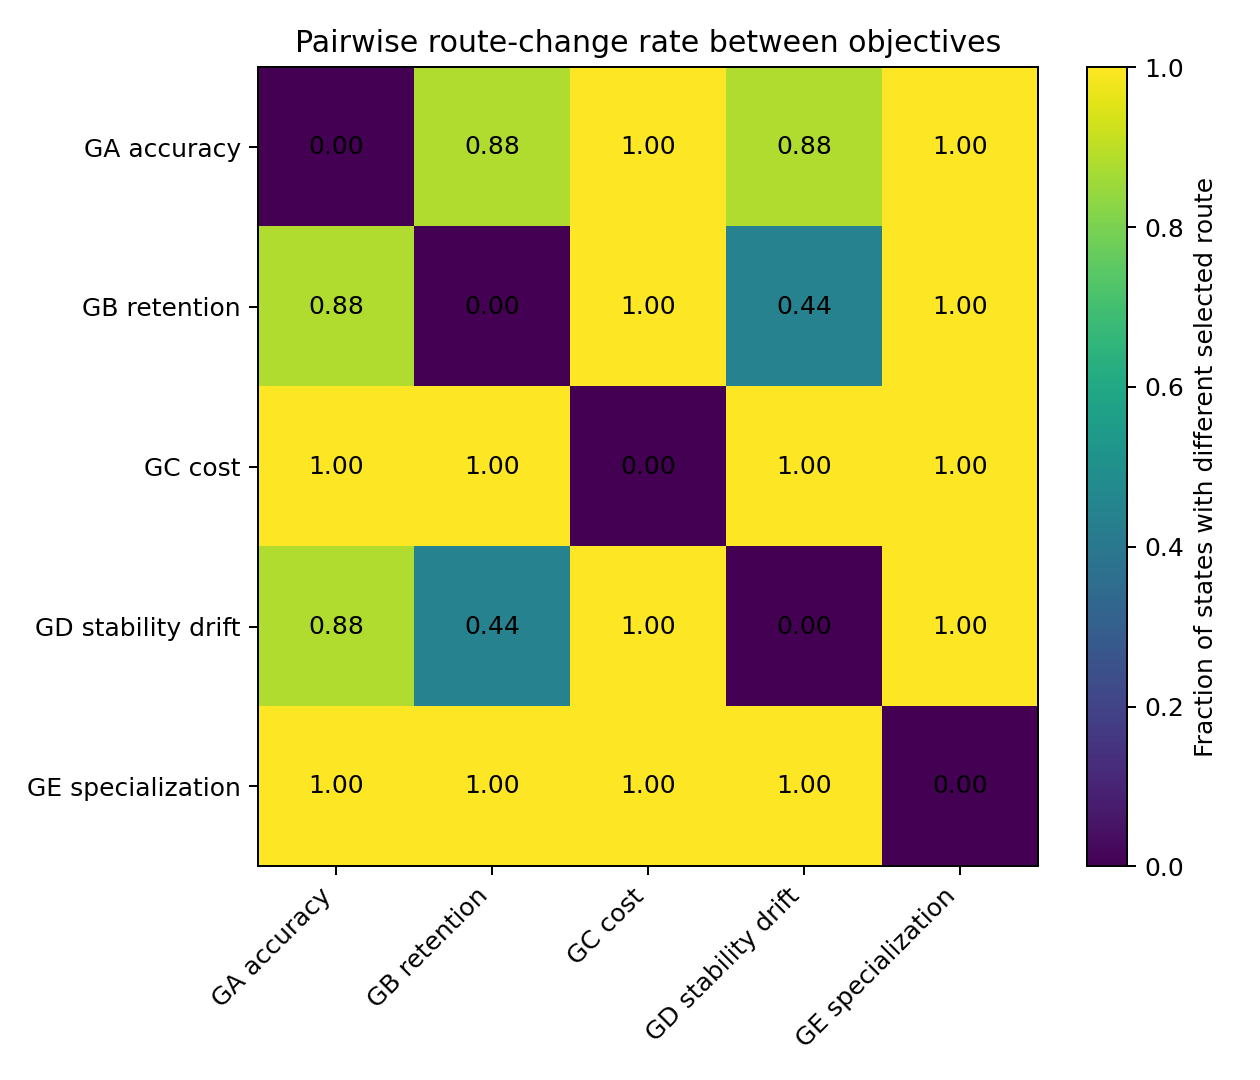
\includegraphics[width=0.72\linewidth]{figures/pairwise_goal_route_change_heatmap.png}
\caption{Pairwise route-change matrix across objectives. High values indicate that two goals induce different route policies over the same states.}
\label{fig:heatmap}
\end{figure}

\subsection{Trade-offs exposed by the controller}
Figure~\ref{fig:tradeoff} shows that the controller exposes trade-offs rather than hiding them. For example, the accuracy objective achieves high accuracy but has a non-zero retention violation rate. This is not a failure of instrumentation; it is evidence that objective-conditioned routing makes trade-offs explicit and therefore auditable.

\begin{figure}[H]
\centering
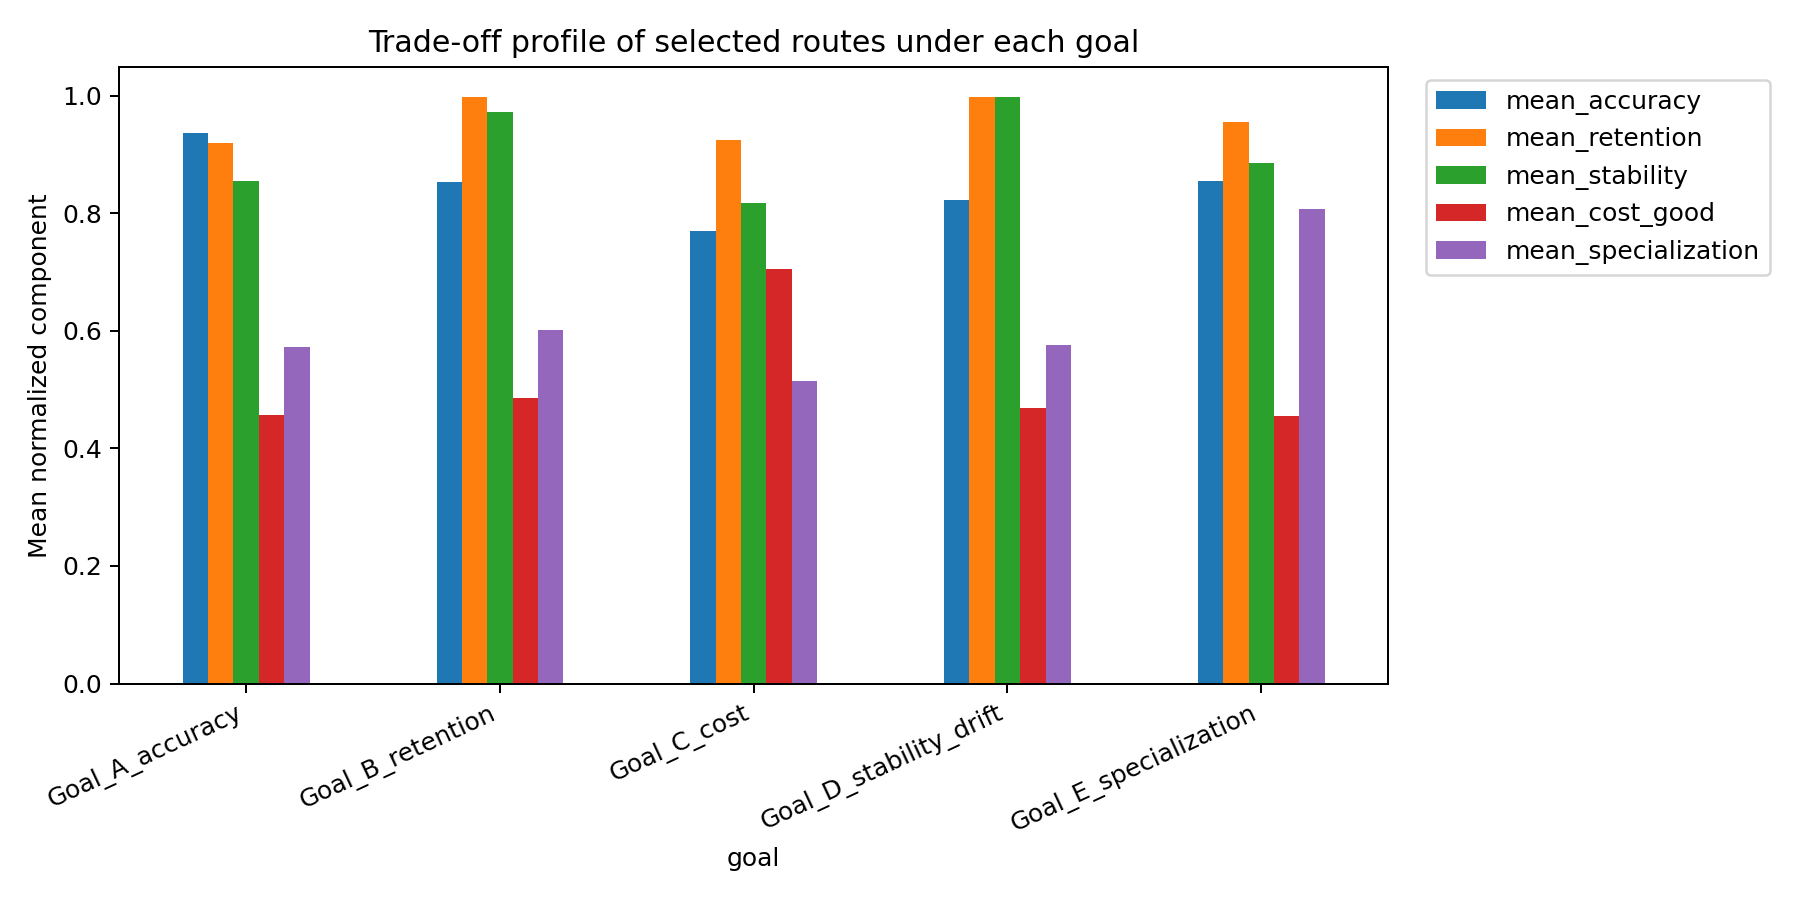
\includegraphics[width=0.92\linewidth]{figures/component_tradeoff_by_goal.png}
\caption{Component trade-off by goal. The goal-adaptive controller optimizes different components depending on the objective vector.}
\label{fig:tradeoff}
\end{figure}

\subsection{Dynamic goal switching}
Figure~\ref{fig:timeline} shows a synthetic timeline in which the active goal changes over time. The adaptive controller changes actions frequently and accumulates higher goal-specific utility than fixed RC2O under the same sequence.

\begin{figure}[H]
\centering
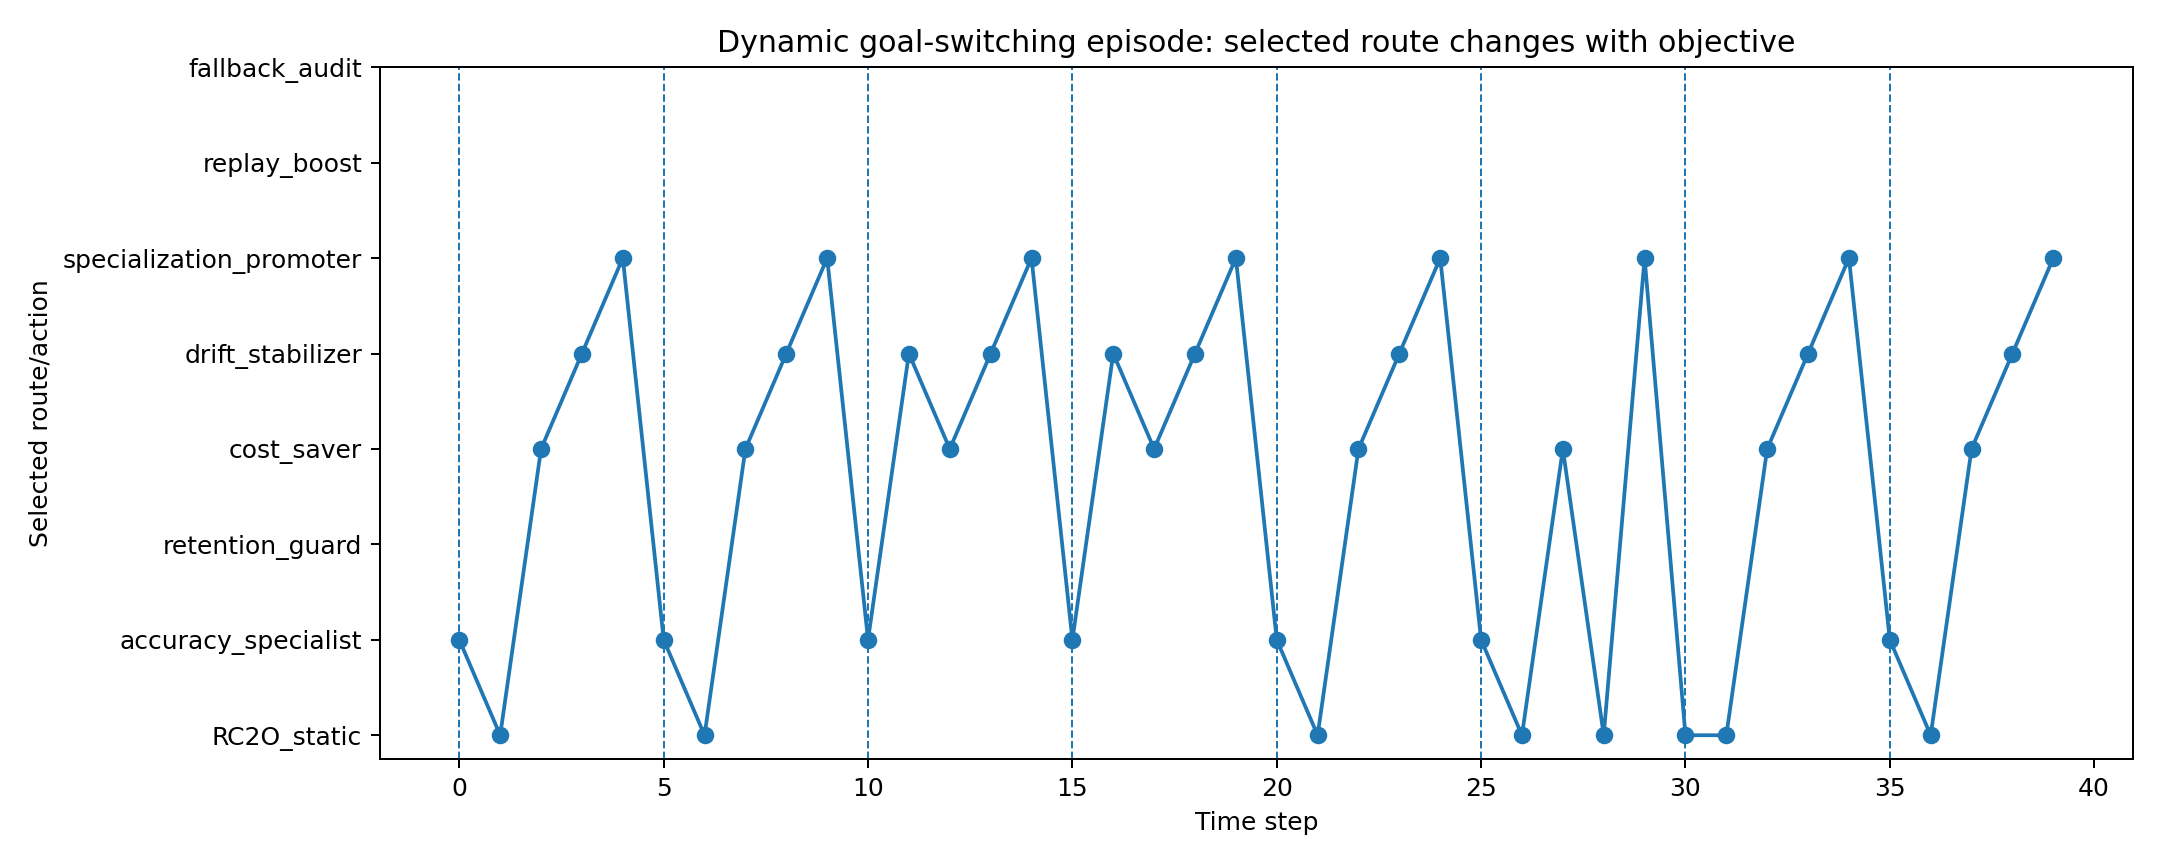
\includegraphics[width=0.96\linewidth]{figures/dynamic_goal_switching_timeline.png}
\caption{Dynamic goal switching timeline. The route changes as the objective changes, supporting the meta-control interpretation.}
\label{fig:timeline}
\end{figure}

\section{Interpretation}
The smoke run supports three claims and rejects a stronger one.

\paragraph{Claim 1: goal-conditioned route differentiation.}
Under the same synthetic states, different objectives induce different route distributions. This is the core result.

\paragraph{Claim 2: RC2O remains the validated core.}
The retention goal remains close to RC2O-like conservative routing. This is desirable: the new controller should not erase the value of RC2O, but expose when other objectives require different choices.

\paragraph{Claim 3: the geometry/RL/FB layers are instrumented.}
The experiment now has explicit state vectors, action scores, goal vectors, route-change metrics, pairwise differentiation metrics, and dynamic goal-switching traces.

\paragraph{Rejected overclaim: universal-control performance.}
The evidence is synthetic. It does not prove real 8-dataset superiority or formal universal control. It demonstrates that the experimental scaffold is ready to consume real RC2O traces.

\section{Connecting to the real MMALS backbone}
The next step should be read-only integration with the real MMALS backbone:
\begin{enumerate}[leftmargin=*]
    \item train/evaluate the real RC2O-8D backbone normally;
    \item export candidate traces with accuracy, retention, stability, cost, entropy, host dominance, specialization and drift metrics;
    \item apply the goal-adaptive controller post-hoc;
    \item compare goal-conditioned route distributions against fixed RC2O;
    \item only later test online or end-to-end control.
\end{enumerate}
This separation keeps the continual-learning evidence clean while allowing the new control layer to be evaluated.

\section{Limitations}
\begin{itemize}[leftmargin=*]
    \item The traces are synthetic and should not be interpreted as real RC2O-8D results.
    \item The forward vector $F(s,a)$ is engineered from audit metrics, not learned end-to-end.
    \item The geometry is an audit geometry, not a proven Riemannian or Lie-group structure.
    \item The RL layer is currently a meta-control formulation and scoring mechanism, not a fully trained online RL agent.
    \item The cost, retention and stability penalties are adjustable and require calibration on real traces.
\end{itemize}

\section{Conclusion}
This work provides a reproducible smoke package for a goal-adaptive MMALS extension. It preserves RC2O as the continual-learning core, adds a measurable audit geometry, formulates routing as a meta-control problem, and introduces a forward-backward objective alignment layer. The central result is route differentiation under changing objectives: accuracy, retention, cost, drift stability, and host specialization induce different routing policies over the same states. The strongest safe conclusion is that the scaffold is ready for post-hoc evaluation on real MMALS RC2O-8D traces.

\section*{Artifact package}
The accompanying package contains:
\begin{itemize}[leftmargin=*]
    \item the compiled PDF and LaTeX source;
    \item all PNG figures;
    \item all CSV outputs;
    \item the Colab notebook;
    \item the generated smoke report;
    \item a README and reproduction notes.
\end{itemize}

\begin{thebibliography}{99}

\bibitem{barreto2017successor}
A. Barreto, W. Dabney, R. Munos, J. Hunt, T. Schaul, D. Silver, and H. van Hasselt.
\newblock Successor features for transfer in reinforcement learning.
\newblock In \emph{Advances in Neural Information Processing Systems}, 2017.

\bibitem{kirkpatrick2017ewc}
J. Kirkpatrick, R. Pascanu, N. Rabinowitz, J. Veness, G. Desjardins, A. A. Rusu, K. Milan, J. Quan, T. Ramalho, A. Grabska-Barwinska, D. Hassabis, C. Clopath, D. Kumaran, and R. Hadsell.
\newblock Overcoming catastrophic forgetting in neural networks.
\newblock \emph{Proceedings of the National Academy of Sciences}, 114(13):3521--3526, 2017.

\bibitem{labsir2026filtering}
S. Labsir, S. El Bouch, C. J. Bordin Jr., and M. G. S. Bruno.
\newblock Filtering and machine learning on Riemannian manifolds and Lie groups.
\newblock \emph{Signal Processing}, 238:110114, 2026.

\bibitem{lessmann2008benchmarking}
S. Lessmann, B. Baesens, C. Mues, and S. Pietsch.
\newblock Benchmarking classification models for software defect prediction: A proposed framework and novel findings.
\newblock \emph{IEEE Transactions on Software Engineering}, 34(4):485--496, 2008.

\bibitem{li2016lwf}
Z. Li and D. Hoiem.
\newblock Learning without forgetting.
\newblock In \emph{European Conference on Computer Vision}, pages 614--629, 2016.

\bibitem{lopezpaz2017gem}
D. Lopez-Paz and M. Ranzato.
\newblock Gradient episodic memory for continual learning.
\newblock In \emph{Advances in Neural Information Processing Systems}, 2017.

\bibitem{musa1987software}
J. D. Musa, A. Iannino, and K. Okumoto.
\newblock \emph{Software Reliability: Measurement, Prediction, Application}.
\newblock McGraw-Hill, 1987.

\bibitem{rothermel2001prioritizing}
G. Rothermel, R. H. Untch, C. Chu, and M. J. Harrold.
\newblock Prioritizing test cases for regression testing.
\newblock \emph{IEEE Transactions on Software Engineering}, 27(10):929--948, 2001.

\bibitem{rusu2016pnn}
A. A. Rusu, N. C. Rabinowitz, G. Desjardins, H. Soyer, J. Kirkpatrick, K. Kavukcuoglu, R. Pascanu, and R. Hadsell.
\newblock Progressive neural networks.
\newblock arXiv:1606.04671, 2016.

\bibitem{sutton2018rl}
R. S. Sutton and A. G. Barto.
\newblock \emph{Reinforcement Learning: An Introduction}.
\newblock MIT Press, second edition, 2018.

\bibitem{touati2021fb}
A. Touati and Y. Ollivier.
\newblock Learning one representation to optimize all rewards.
\newblock In \emph{Advances in Neural Information Processing Systems}, 2021.

\bibitem{touati2022zeroshot}
A. Touati, J. Rapin, and Y. Ollivier.
\newblock Does zero-shot reinforcement learning exist?
\newblock arXiv:2209.14935, 2022.

\end{thebibliography}

\end{document}
